\documentclass[11pt]{beamer}
\usetheme{Warsaw}
\setbeamertemplate{footline}[frame number]
\setbeamertemplate{navigation symbols}{} %no nav symbols
\usepackage{color}
\usepackage{amsmath,amssymb}
%\usepackage{amssymb}
\usepackage{lmodern} % same visually appearance as the default ``Computer Modern'' but with better beamer compatability (more font sizes)
\usepackage{stackrel}
\usepackage{graphicx}
\usepackage[]{caption}
\usepackage[]{subcaption}
%\usepackage{verbatim}
\useoutertheme{progressbar}

\renewcommand{\L}{\LaTeX\ }
\title{Posters in \L\ }
\author[Jordan Roberts]{\textsc{Jordan Roberts}}
\institute{\textsc{Department of Mechanical Engineering\\Auburn University}}
\date[7/26/2010]{\textsc{\scriptsize{July 26, 2010}}}



\begin{document}


%%%%%%%%%%%%%%%%%%%%%%%%%%%%%%Frame 1

\maketitle
%%%%%%%%%%%%%%%%%%%%%%%%%%%%%%%%%%%% Frame 2
\begin{frame}[shrink]{Outline}{}
{%\footnotesize 
%\begin{columns}
%\begin{column}[t]{0.5\textwidth}
\tableofcontents[sections={1-5}]
%\end{column}
%\begin{column}[t]{0.5\textwidth}
%\tableofcontents[sections={4-5}]
%\end{column}
%\end{columns}
}
\end{frame}

%%%%%%%%%%%%%%%%%%%%%%%%%%%%%%Frame 3
\section{Introduction}
\subsection{Paper Basics}
\begin{frame}[fragile,shrink]
\frametitle{Paper}\framesubtitle{Basics}
	\centering
	\begin{figure}[htbp]
		\includegraphics[scale=.15]{Asizeillustration.pdf}
		\caption{ISO 216 A Series Paper}
		\label{fig:apaper}
	\end{figure}
\end{frame}

%%%%%%%%%%%%%%%%%%%%%%%%%%%%%%Frame 4
%\section{Introduction}
\subsection{Options}
\begin{frame}[fragile,shrink]
\frametitle{\L\ Posters}\framesubtitle{Options}
Options for Creating Posters in \L
			\begin{itemize}
				\item \verb|baposter| class
				\item \verb|a0poster| class
				\item \verb|beamerposter| package
			\end{itemize}
\end{frame}

%%%%%%%%%%%%%%%%%%%%%%%%%%%%%%Frame 5
\section{baposter}
\subsection{Background}
\begin{frame}[fragile,shrink]
\frametitle{baposter}\framesubtitle{Background}
	\verb|baposter| class
			\begin{itemize}
				\item created and maintained by Brian Amberg
				\item most posters look the same
				\item limited options
				\item seems to be the least supported option
			\end{itemize}
		Downloads and documentation can be found here:  \url{http://www.brian-amberg.de/uni/poster/}
\end{frame}

%%%%%%%%%%%%%%%%%%%%%%%%%%%%%%Frame 6
\begin{frame}[fragile,shrink]
\frametitle{baposter}\framesubtitle{Example Output}
	\begin{figure}[htbp]
		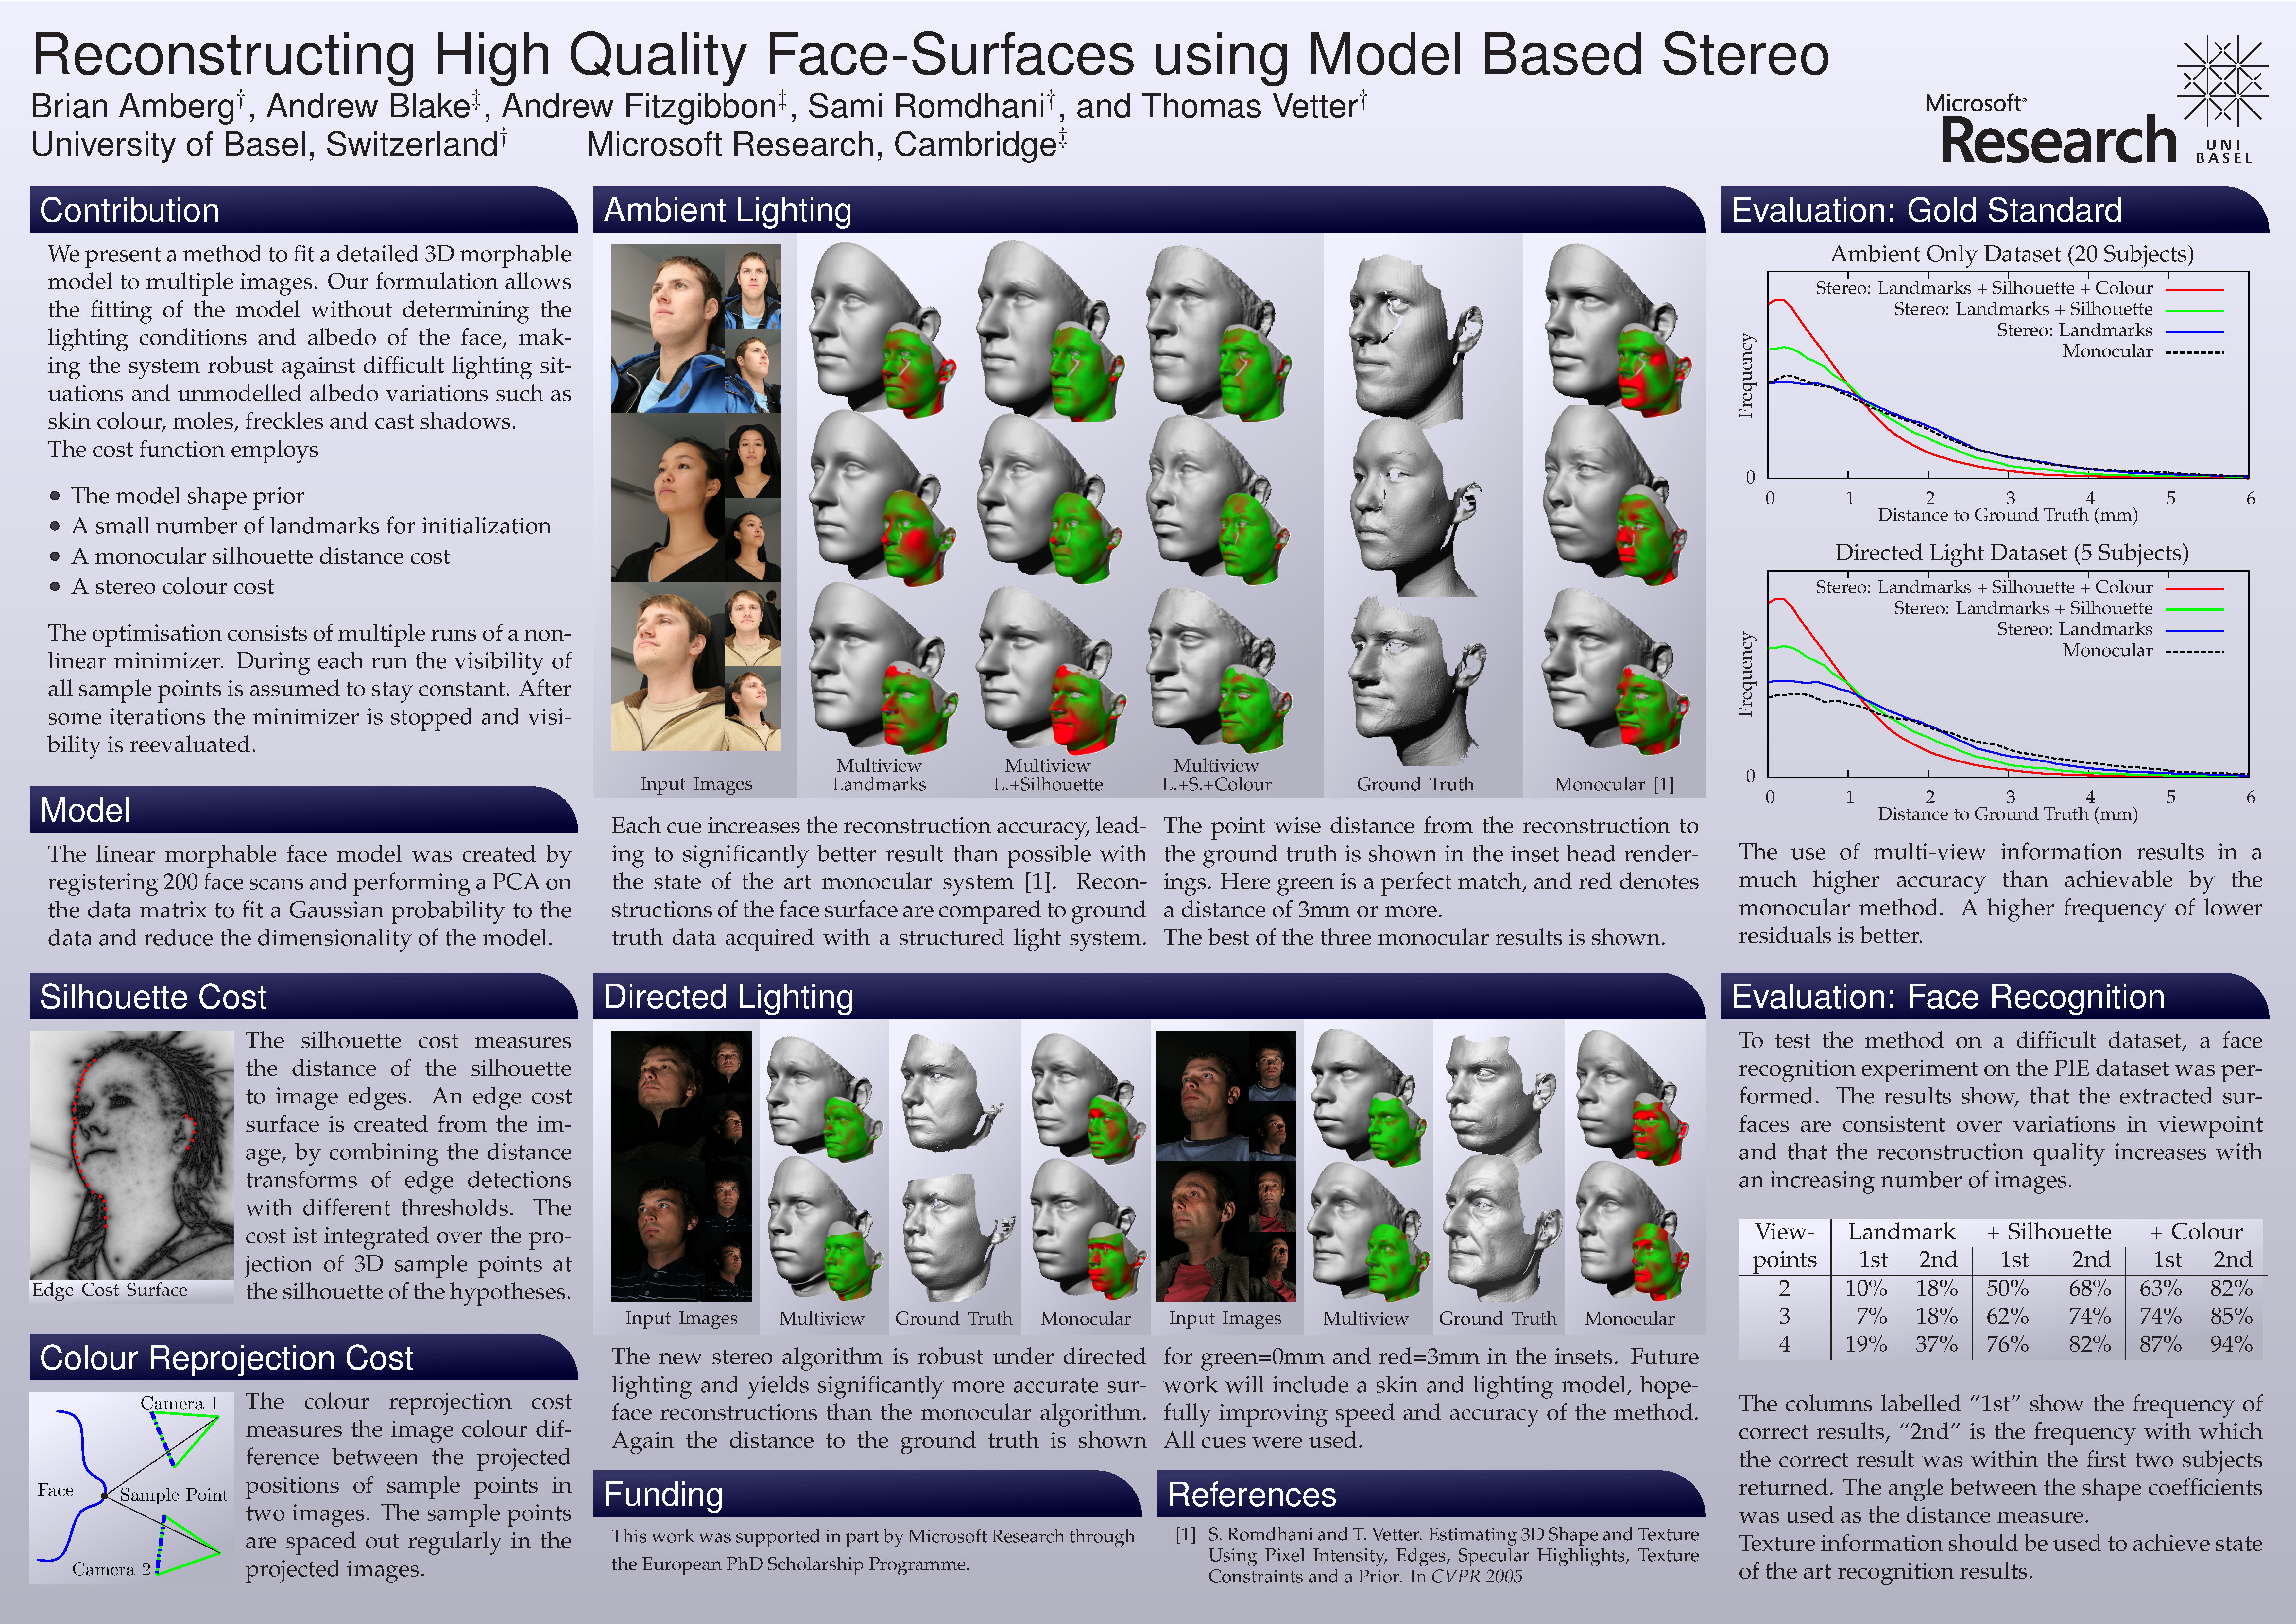
\includegraphics[scale=.06]{baposterex1.pdf}
		\caption{baposter example}
		\label{fig:baex1}
	\end{figure}
\end{frame}


%%%%%%%%%%%%%%%%%%%%%%%%%%%%%%Frame 7
\begin{frame}[fragile,shrink]
	\frametitle{baposter}\framesubtitle{Usage}
\begin{itemize}
	\item Works with:
		\begin{itemize}
				\item miktek 2.7
				\item texlive 2007
		\end{itemize}
	\item Does \emph{\emph{not}} work with:
			\begin{itemize}
				\item miktek 2.2
				\item older versions of tetex
				\item \emph{possibly} older versions of pgf
				\item \verb|xkeyvals| older than v2.5
		\end{itemize}
\end{itemize}
\end{frame}


%%%%%%%%%%%%%%%%%%%%%%%%%%%%%%Frame 8
\section{a0poster}
\subsection{Background}
\begin{frame}[fragile,shrink]
\frametitle{a0poster}\framesubtitle{Background}
	\verb|a0poster| class
			\begin{itemize}
				\item developed by Gerlinde Kettl and Matthias Weiser
				\item Composed of four files
				\begin{itemize}
					\item \verb|a0poster.cls| Defines the class file
					\item \verb|a0size.sty|		Defines the font sizes
					\item \verb|a0_eng.tex|		Manual in English
					\item \verb|a0.tex|				Manual in German
				\end{itemize}
				\item font sizes 12pt \verb|(\tiny)| up to 107 pt \verb|(\VERYHuge)|	
			\end{itemize}
		Downloads and documentation can be found here:  \url{http://www.ctan.org/tex-archive/help/Catalogue/entries/a0poster.html}
\end{frame}


%%%%%%%%%%%%%%%%%%%%%%%%%%%%%%Frame 9
%\subsection{Background}
\begin{frame}[fragile,shrink]
\frametitle{a0poster}\framesubtitle{Pitfalls}
				\begin{itemize}
					\item Claims to work with A0, A1, A2, A3, and A4
					\item Has issues with scaling to sizes other than A0
						\begin{itemize} \item \emph{may} have been fixed with latest revision \end{itemize}
					\item	requires absolute positioning
					\item \emph{they} prefer \L\ to pdf\L\ to take advantage of PStricks
			\end{itemize}
\end{frame}

%%%%%%%%%%%%%%%%%%%%%%%%%%%%%%Frame 10
%\subsection{Background}
\begin{frame}[fragile,shrink]
\frametitle{a0poster}\framesubtitle{Things to know}
			\begin{itemize}
				\item \verb|a0poster.cls| based on article class
				\item \verb|a0header.ps| file is created used by dvips to manage size
				\item \verb|a0poster| does not support colors or pictures without pstricks etc.
			\end{itemize}
\end{frame}


%%%%%%%%%%%%%%%%%%%%%%%%%%%%%%Frame 11
%\subsection{Background}
\begin{frame}[fragile,shrink]
\frametitle{a0poster}\framesubtitle{Usage}
		\begin{block}{Sample Code}
			%\begin{verbatim}
			\texttt{\textbackslash documentclass[portrait,a0,final]\{a0poster\}}\\
			 \texttt{\textbackslash begin\{document\} }\\
			   \texttt{\% Write poster here}\\
			 	\texttt{\textbackslash end\{document\}}
		%\end{verbatim}
		\end{block}		
		Replace \verb|portrait| with \verb|landscape|  to be in landscape mode.
\end{frame}



%%%%%%%%%%%%%%%%%%%%%%%%%%%%%%Frame 12
%\subsection{Background}
\begin{frame}[fragile,shrink]
\frametitle{a0poster}\framesubtitle{Usage}
		\begin{block}{a0poster class options}
		\footnotesize
			\begin{tabular}{l l}
				\verb|landscape| & landscape format \textbf{(default)}\\
				\verb|portrait| & portrait format\\
				\verb|a0b| & DIN A0 big. Full width of HP Designjet 650C \textbf{(default)}\\
				\verb|a0| & DIN A0\\
				\verb|a1| & DIN A1\\
				\verb|a2| & DIN A2\\
				\verb|a3| & DIN A3\\
				\verb|draft| & reduces PS output to DIN A4 size\\
				\verb|final| & PS output in original size \textbf{(default)}\\
			\end{tabular}
		\normalsize
			
		\end{block}		
		
\end{frame}

%%%%%%%%%%%%%%%%%%%%%%%%%%%%%%Frame 13
%\subsection{Background}
\begin{frame}[fragile,shrink]
\frametitle{a0poster}\framesubtitle{Usage}
		\begin{block}{a0poster font size options}
		\footnotesize
			\begin{tabular}{l l}
				\textbackslash \verb|tiny| & 12pt\\
				\textbackslash \verb|scriptsize| & 14.4pt\\
				\textbackslash \verb|footnotesize| & 17.28pt\\
				\textbackslash \verb|small| & 20.74pt\\
				\textbackslash \verb|normalsize| & 24.88pt\\
				\textbackslash \verb|large| & 29.86pt\\
				\textbackslash \verb|Large| & 35.83pt\\
				\textbackslash \verb|LARGE| & 43pt\\
				\textbackslash \verb|huge| & 51.6pt\\
				\textbackslash \verb|Huge| & 61.92pt\\
				\textbackslash \verb|veryHuge| & 74.3pt\\
				\textbackslash \verb|VeryHuge| & 89.16pt\\
				\textbackslash \verb|VERYHuge| & 107pt\\
			\end{tabular}
		\normalsize
			
		\end{block}		
		
\end{frame}


%%%%%%%%%%%%%%%%%%%%%%%%%%%%%%Frame 14
%\subsection{Background}
\begin{frame}[fragile,shrink]
\frametitle{a0poster}\framesubtitle{Usage}
		\begin{block}{a0poster positioning}
			\begin{itemize}
				\item Positioning is done by order of code. Unless\ldots
				\item you use the \verb|textpos| package
				\item \textbackslash \verb|usepackage[absolute,overlay]{textpos}|
		\end{itemize}
					
		\end{block}		
		\footnotesize
		\begin{block}{textpos options}
				\begin{tabular}{ l l }
					absolute & makes origin upper left corner\\
					overlay & gives text blocks opaque backgrounds\\
					\textbackslash \verb|textblockcolour{color_name}| & changes color of background\\
					showboxes & draws rectangle around text block\\
				\end{tabular}	
		\end{block}
		
\end{frame}


%%%%%%%%%%%%%%%%%%%%%%%%%%%%%%Frame 15
%\subsection{Background}
\begin{frame}[fragile,shrink]
\frametitle{a0poster}\framesubtitle{Usage}
		\begin{block}{textblock usage}
				\texttt{\textbackslash begin\{textblock\}\{hsize\}(hpos, vpos) }\\
					Some text\\
				\texttt{\textbackslash end\{textblock\}}\\
		\end{block}		
	\verb|hsize| and \verb|hpos| given in units of module \textbackslash \verb|TPHorizModule| \\
	\verb|vpos| based on module \textbackslash \verb|TPVertModule|
			\begin{block}{textblock usage}
				\texttt{\textbackslash begin\{textblock\}\{20.5\}(1.5, 2.5)}\\
					Some text\\
				\texttt{\textbackslash end\{textblock\}}\\
		\end{block}	
		
\end{frame}

%%%%%%%%%%%%%%%%%%%%%%%%%%%%%%Frame 16
%\subsection{Background}
\begin{frame}[fragile,shrink]
\frametitle{a0poster}\framesubtitle{Usage}
 We define \textbackslash \verb|TPHorizModule| and \textbackslash \verb|TPVertModule| in the preamble as follows
			\begin{block}{textblock usage}
				\texttt{\textbackslash setlength\{\textbackslash TPHorizModule\}\{1cm\}}\\
				\texttt{\textbackslash setlength\{\textbackslash TPVertModule\}\{1cm\}}	
			\end{block}	
We can also place a grid with \texttt{\textbackslash includepackage[colorgrid,texcoord]\{eso-pic\}}	
\end{frame}


%%%%%%%%%%%%%%%%%%%%%%%%%%%%%%Frame 17
\section{beamerposter}
\subsection{Background}
\begin{frame}[fragile,shrink]
\frametitle{beamerposter}\framesubtitle{Background}
			\begin{itemize}
				\item \L \verb|beamerposter| package
				\item Created by Philippe Dreuw and Thomas Deselaers
				\item Extension of \verb|beamer|  and \verb|a0poster| class
				\item Creates posters in DIN-AX sizes and custom sizes
				\item applicable to custom beamer slides
			\end{itemize}
\end{frame}

%%%%%%%%%%%%%%%%%%%%%%%%%%%%%%Frame 18
\subsection{Basics}
\begin{frame}[fragile,shrink]
\frametitle{\L\ Requirements}%\framesubtitle{blank}
			\begin{itemize}
				\item \verb|beamer| class
				\item \verb|fp| package (in version supporting choice keys, e.g. v2.5f
				\item \verb|type1cm| package for scalable and huge math fonts
			\end{itemize}
\end{frame}
 

%%%%%%%%%%%%%%%%%%%%%%%%%%%%%%Frame 19
\begin{frame}[fragile,shrink]
\frametitle{beamerposter}\framesubtitle{downloads}
			\begin{itemize}
				\item \verb|beamerposter| package available several places:
				\begin{itemize}
					\item \url{http://tug.ctan.org/cgi-bin/ctanPackageInformation.py?id=beamerposter}
				\item \url{http://tug.ctan.org/tex-archive/macros/latex/contrib/beamerposter/}
				\end{itemize}
				\item google group \url{http://groups.google.com/group/beamerposter}
			\end{itemize}
\end{frame}

%%%%%%%%%%%%%%%%%%%%%%%%%%%%%%Frame 20
\begin{frame}[fragile,shrink]
\frametitle{beamerposter}\framesubtitle{versions}
			\begin{itemize}
				\item Current version of \verb|beamerposter| package is 1.11
				\item ProTeXt release has v1.07
				\item Release Notes:
					\begin{itemize}
						\item \verb|beamerposter.sty.111| - renived uncompatible paralist package, bugfixed list indention problem
						\item \verb|beamerposter.sty.110| - improved package errors, warnings, and info messages
						\item \verb|beamerposter.sty.109| - bugfixed list indentation problem (e.g. itemize/enumerate/description/etc.), added printer option for external printer definition files
						\item \verb|beamerposter.sty.108| - supports external printer definition files, added grid mode option, renamed beamer specific variables, added font size normalization (scale=1.0 is now default for all DIN-A(n) sizes)
					\end{itemize}
			\end{itemize}
\end{frame}





%%%%%%%%%%%%%%%%%%%%%%%%%%%%%%Frame 21
\begin{frame}[fragile,shrink]
\frametitle{\texttt{beamerposter} EXAMPLE CODE}%\framesubtitle{blank}
		\begin{verbatim}
			\documentclass[final,hyperref={pdfpagelabels=false}]{beamer} 
  \mode<presentation> {  %% check http://www-i6.informatik.rwth-aachen.de/~dreuw/latexbeamerposter.php for examples
    \usetheme{Berlin}    %% you should define your own theme e.g. for big headlines using your own logos 
  }
  \usepackage[english]{babel}
  \usepackage[latin1]{inputenc}
  \usepackage{amsmath,amsthm, amssymb, latexsym}
  %\usepackage{times}\usefonttheme{professionalfonts}  % times is obsolete
  \usefonttheme[onlymath]{serif}
  \boldmath
  \usepackage[orientation=portrait,size=a0,scale=1.4,debug]{beamerposter}                       % e.g. for DIN-A0 poster
  %\usepackage[orientation=portrait,size=a1,scale=1.4,grid,debug]{beamerposter}                  % e.g. for DIN-A1 poster, with optional grid and debug output
  %\usepackage[size=custom,width=200,height=120,scale=2,debug]{beamerposter}                     % e.g. for custom size poster
  %\usepackage[orientation=portrait,size=a0,scale=1.0,printer=rwth-glossy-uv.df]{beamerposter}   % e.g. for DIN-A0 poster with rwth-glossy-uv printer check
  % ...
  %
  \title[Fancy Posters]{Making Really Fancy Posters with \LaTeX}
  \author[Dreuw \& Deselaers]{Philippe Dreuw and Thomas Deselaers}
  \institute[RWTH Aachen University]{Human Language Technology and Pattern Recognition,RWTH Aachen University}
  \date{Jul. 31th, 2007}
  \begin{document}
  \begin{frame}{} 
    \vfill
    \begin{block}{\large Fontsizes}
      \centering
      {\tiny tiny}\par
      {\scriptsize scriptsize}\par
      {\footnotesize footnotesize}\par
      {\normalsize normalsize}\par
      {\large large}\par
      {\Large Large}\par
      {\LARGE LARGE}\par
      {\veryHuge veryHuge}\par
      {\VeryHuge VeryHuge}\par
      {\VERYHuge VERYHuge}\par
    \end{block}
    \vfill
  \end{frame}
  \end{document}


		\end{verbatim}
\end{frame}

%%%%%%%%%%%%%%%%%%%%%%%%%%%%%%Frame 22
\begin{frame}[fragile,shrink]
\frametitle{\texttt{beamerposter} Example}%\framesubtitle{blank}
		\begin{figure}[htbp]
	\centering
	\includegraphics[scale=.05]{BPEX1.pdf}
	\caption{Simple beamerposter output}
	\label{fig:easy1}
\end{figure}	
	
\end{frame}

%%%%%%%%%%%%%%%%%%%%%%%%%%%%%%Frame 23
\begin{frame}[fragile,shrink]
\frametitle{Questions?} 
		
		%``So don't ask me no questions, and I won't tell you no lies.''-Ronnie VanZant
		\href{http://www.youtube.com/watch?v=DCfWmNJt4D4}{``So don't ask me no questions, and I won't tell you no lies.''-Ronnie VanZant}	
	
\end{frame}

%%%%%%%%%%%%%%%%%%%%%%%%%%%%%%Frame 23
\begin{frame}[fragile,shrink]
\frametitle{HW} 
	
	Using any of the three packages discussed, successfully compile any example poster.  Submit code and poster printout using a ``fit to paper'' command in adobe or your choice of pdf or ps viewer.	
		
\end{frame}




\end{document}